\documentclass[12pt,a4paper]{report}

\usepackage[left=1.5in,right=1in,top=1.5in,bottom=1in]{geometry}
\usepackage{mathptmx}
\usepackage[T1]{fontenc}
\usepackage[utf8]{inputenc}
\usepackage{setspace}
\onehalfspacing
\usepackage{titlesec}
\usepackage{graphicx}
\usepackage{booktabs}
\usepackage{multirow}
\usepackage{amsmath}
\usepackage{amssymb}
\usepackage[font=footnotesize,labelfont=bf]{caption}
\usepackage[round]{natbib}
\usepackage[hidelinks]{hyperref}

\titleformat{\chapter}[display]
  {\normalfont\centering\bfseries\fontsize{14}{17}\selectfont}
  {CHAPTER \thechapter:}{0.5ex}{\fontsize{14}{17}\selectfont}
\titlespacing*{\chapter}{0pt}{0pt}{18pt}
\titleformat{\section}{\normalfont\bfseries\fontsize{12}{15}\selectfont}{\thesection}{1em}{}
\titleformat{\subsection}{\normalfont\bfseries\fontsize{12}{15}\selectfont}{\thesubsection}{1em}{}

\begin{document}

% ---------------------------------------------------------------------------
% Title page
% ---------------------------------------------------------------------------
\begin{titlepage}
\thispagestyle{empty}
\begin{center}
{\large UNIVERSITY OF MACAU}\\[0.2cm]
{\large Faculty of Science and Technology}\\[0.2cm]
{\large Department of Computer Science}\\[1.2cm]
{\Large\bfseries From Prompting to Structured Alignment:\\[0.2cm]
Individual, Population, and Temporal Boundaries of\\[0.2cm]
LLM Survey Simulation}\\[1.2cm]
by\\[0.3cm]
{\large CHENYU YUAN}\\[1.2cm]
A thesis submitted in partial fulfillment of the requirements for the degree of\\[0.3cm]
{\large Master of Computer Science}\\[1.2cm]
Thesis Supervisor: PENGYANG WANG\\[1.2cm]
April 2027
\end{center}
\end{titlepage}

% ---------------------------------------------------------------------------
% Front matter
% ---------------------------------------------------------------------------
\pagenumbering{roman}
\setcounter{page}{2}

\chapter*{Abstract}
\addcontentsline{toc}{chapter}{Abstract}
\begin{center}
{\large University of Macau}\\[0.6cm]
{\bfseries From Prompting to Structured Alignment: Individual, Population, and Temporal Boundaries of LLM Survey Simulation}\\[0.4cm]
by\\[0.2cm]
CHENYU YUAN\\[0.3cm]
Thesis Supervisor: PENGYANG WANG
\end{center}

\vspace{0.4cm}

Large language models are increasingly used as virtual survey respondents, but
most evaluations treat surveys as one-shot prompting tasks. This thesis presents
a data-centric pipeline that reconstructs voter--candidate interactions from the
American National Election Studies (ANES), aligns a compact 8B model with survey
distributions through LoRA fine-tuning, and evaluates the resulting model at the
individual, population, and temporal levels. On unseen respondents in the
2016--2019 waves, the fine-tuned model reaches a mean absolute error of 20.84, a
correlation of 0.679, and a rating-induced choice accuracy of 0.518 against a
chance level of 0.163. A gradient-boosted baseline on the same features reaches
20.58, 0.714, and 0.534; paired bootstrap shows no significant difference in MAE
or choice, while the baseline has a higher correlation. On General Social Survey
policy attitudes, fine-tuning reduces marginal and joint Jensen--Shannon
divergence by 91\% and 86\% on the EDC configuration. The thesis then reports a
sharp temporal boundary: individual-level correlation falls from 0.722 in 2019
to near zero in 2024, and both the language model and the tabular baseline
collapse in 2024. Adding the 2022 wave to training does not help. The results
suggest that structured alignment is necessary but not sufficient for social
simulation, and that temporal distribution shift should be treated as a
first-class evaluation axis.

\clearpage
\tableofcontents
\clearpage
\listoffigures
\clearpage
\listoftables
\clearpage

\chapter*{List of Abbreviations}
\addcontentsline{toc}{chapter}{List of Abbreviations}
\begin{tabular}{ll}
ANES & American National Election Studies \\
ECE & Expected Calibration Error \\
FAS & Full Attribute Simulation \\
GSS & General Social Survey \\
IPF & Iterative Proportional Fitting \\
JS & Jensen--Shannon divergence \\
KL & Kullback--Leibler divergence \\
LLM & Large Language Model \\
LoRA & Low-Rank Adaptation \\
MAE & Mean Absolute Error \\
PAS & Partial Attribute Simulation \\
RMSE & Root Mean Squared Error \\
\end{tabular}

% ---------------------------------------------------------------------------
% Main body
% ---------------------------------------------------------------------------
\clearpage
\pagenumbering{arabic}

\chapter{Introduction}
\label{ch:intro}

Questionnaire surveys are a primary source of evidence in the social sciences and
in public policy, but they are expensive, slow, and difficult to field at scale.
Large language models (LLMs) have been proposed as virtual survey respondents:
given a demographic profile and a question, a model can produce an answer without
recruiting a participant \citep{argyle2022,dillion2023,kim2023}. Most existing
work evaluates the model as a one-shot prompt. A profile is placed in the context
window, a question is asked, and the answer is scored. This measures how well a
model can role-play a respondent in a single turn. It does not test whether the
model has internalized the structure of survey responses, whether its outputs are
coherent at the population level, or whether the behaviour survives a change in
the political environment.

This thesis takes a data-centric view. Survey responses are generated by a
structured process: partisan identity, ideological position, and demographics
interact with the attributes of a candidate, and the resulting evaluations follow
regularities that are stable within an era but can shift across eras. If an LLM
is to act as a credible respondent, it should be trained on that structure rather
than prompted with it. The thesis reconstructs voter--candidate interactions from
the American National Election Studies (ANES), aligns a compact 8B model with the
resulting distribution through LoRA fine-tuning, and evaluates the model at the
individual, population, and temporal levels.

The thesis makes four contributions. First, it provides a reproducible data
construction and audit. The raw ANES table contains duplicate thermometer items
stored under trailing-period names (\texttt{obama.} and \texttt{obama}) and
social-group thermometers stored in the same column as candidate thermometers.
Both defects are quantified and removed, reducing 132,948 raw rows to 98,159
clean interaction-level rows. Because ANES is a panel (3,080 of 3,165 respondents
appear in more than one wave, and there are no test-only respondents in
2022/2024), two complementary protocols are reported: a temporal split and a
respondent-disjoint split.

Second, the thesis reports a conservative individual-level evaluation. On unseen
respondents in 2016--2019, the fine-tuned model reaches an MAE of 20.84, a
correlation of 0.679, and a choice accuracy of 0.518 against chance 0.163. A
gradient-boosted baseline on the same features reaches 20.58, 0.714, and 0.534;
paired bootstrap shows no significant MAE or choice difference, while the
baseline has a higher correlation. The value of the LLM is not superior point
prediction; it is a unified interface that also produces a rating distribution
and extends to population-level generation.

Third, on GSS policy attitudes, fine-tuning reduces marginal and joint
Jensen--Shannon divergence by 91\% and 86\% on the EDC configuration, and by up
to 76\% and 64\% on EHC. The gain comes from supervised fine-tuning, not from
retrieval or quota sampling.

Fourth, the thesis reports a temporal boundary. Across 2016--2024,
individual-level correlation falls from 0.722 in 2019 to $-0.056$ in 2024, and
the tabular baseline collapses in the same way. Adding the 2022 wave to training
does not help. Structured alignment is necessary but not sufficient for social
simulation.

\section{Related Work}

Work on LLMs as virtual respondents conditions models on demographic backstories
and compares the resulting ``silicon samples'' with survey margins
\citep{argyle2022,santurkar2023,dillion2023,kim2023}. Later work extends the
paradigm to random silicon sampling \citep{sun2024}, cross-survey probing
\citep{zhou2024}, multi-domain benchmarks \citep{zhao2025}, and specialization to
survey response distributions \citep{cao2025}. Most of this work evaluates a
model as a one-shot respondent and rarely separates individual accuracy from
population-level alignment.

A related literature studies persona fidelity and personalization
\citep{park2024,wang2024,xu2024,salemi2024,ng2024}. That work is primarily about
behavioural consistency within a conversation; the present setting asks the model
to reproduce the statistical structure of survey responses across a population.
Fine-tuning has also been used to align models with political or social
preferences \citep{chu2023,zhao2023}; here the goal is competence alignment---the
rules that map a profile and a candidate to a rating---rather than adopting a
group's voice. For population-level generation, iterative proportional fitting
\citep{deming1940,fienberg1970} and LOESS \citep{cleveland1979} provide the
classical tools that are combined with the language model.

Prior work on LLM survey simulation has generally evaluated on a single wave or on
a pooled sample, which can hide temporal decay. The per-year analysis in
Chapter~\ref{ch:temporal} reports a monotonic decay for both a fine-tuned LLM and
a feature-engineered baseline on the same ANES panel. This is, to our knowledge,
the first such comparison on a common panel.

\chapter{Data and Methodology}
\label{ch:method}

\section{Data Construction}

The individual-level corpus is built from the ANES pilot waves of 2016, 2018,
2019, 2020, 2022, and 2024 (132,948 rows, 3,165 respondents, 29 candidates). The
population-level component uses the GSS waves of 2004--2022, with 2024 as the
target year. The raw ANES table contains two defects. Trailing-period duplicates
(\texttt{obama.} and \texttt{obama}, \texttt{hrc.} and \texttt{hrc}) produce
8,165 rows; social-group thermometers (\texttt{black}, \texttt{white},
\texttt{dem}, \texttt{rep}) stored in the candidate column produce 23,060 rows.
Names are normalized, candidate and group targets are separated, missing or
out-of-range scores are removed (3,588), and duplicates are dropped (8,141). The
clean candidate table contains 98,159 rows.

Each observation is represented as a triple $(v_i,c_j,y_{ij}\mid t_i)$, where
$v_i$ is the voter profile, $c_j$ the target, $y_{ij}\in[0,100]$ the thermometer,
and $t_i$ the year. Candidate identity is decoupled from attributes: each
candidate is described by a metadata vector $\mathcal{M}[c]$ containing party,
ideology, age, position, and incumbent status. Three features encode social
cognition. Party match is $+1$ for a co-partisan, $-1$ for an independent, and
$0$ otherwise. Ideological distance is the seven-point distance
$\lvert\text{lcself}_v-\text{ideology}_c\rvert\in[0,6]$. A similarity index
combines party, ideology, race, gender, and age with weights
$0.25,0.25,0.20,0.15,0.15$. Cross-pressure indicators flag same-party but
ideologically distant pairs (CP1), different-party but ideologically close pairs
(CP2), and demographically similar but different-party pairs (CP3).

\section{Evaluation Protocols}

ANES is a panel: 3,080 of 3,165 respondents appear in more than one wave, and
every respondent observed in 2022 or 2024 also appears in 2016--2020. There are
zero test-only respondents. A temporal split can therefore measure transfer to a
later wave, but not generalization to unseen individuals. The temporal protocol
(T) trains on 2016--2020 (6,516 rows), validates on 2022 (2,501), and tests on
2024 (3,421). The respondent protocol (R) splits respondents 80/20 by a hash of
the respondent identifier: 5,094 training rows and 6,014 test rows. A strict cell
(T$\times$R) contains the 226 rows from 2024 whose respondents are held out. R is
the main in-distribution test; T measures the temporal boundary.

\section{Fine-Tuning and Readouts}

The model is Qwen3-8B. LoRA is applied to all attention and MLP projections with
rank $r=8$, scaling $\alpha=32$, and dropout $0.1$. Training uses three epochs, a
learning rate of $10^{-4}$, an effective batch size of 16, and a maximum sequence
length of 512. The loss is the causal language-modeling loss on the answer tokens
only; prompt tokens are masked. This yields 21.8M trainable parameters (0.27\% of
the model), and three seeds (42, 43, 44) are used.

Two readouts are used. \emph{Generation} decodes greedily and parses the first
integer in $[0,100]$; it preserves individual variation and is the primary readout
for choice. \emph{Anchor likelihood} scores eleven anchors
$a\in\{0,10,\dots,100\}$ by their sequence log-probability, normalizes with a
softmax, and reports the expectation and the argmax. For choice, the candidate
with the highest predicted score is selected within each respondent--year group;
accuracy is reported against the rating-induced choice and against chance.

\section{Population-Level Pipeline}

For full attribute simulation (FAS), every univariate and pairwise cell is
extrapolated with a four-model ensemble,
\begin{equation}
\hat p(t^*)=\frac{1.0\hat p_{\text{poly}}+1.0\hat p_{\text{loess}}
+0.6\hat p_{\text{exp}}+0.8\hat p_{\text{lin}}}{3.4}.
\end{equation}
The predicted marginals and pairwise tables are combined with iterative
proportional fitting: starting from the independence approximation,
multiplicative updates match each pairwise table and marginal, run for 800
iterations, and are normalized with Laplace smoothing. The resulting joint
distribution is used to generate five task types: batch generation (50\%),
prior-constrained sampling (25\%), scenario variation (15\%), subgroup analysis
(7\%), and iterative correction (3\%).

\section{Metrics}

For PAS, MAE, RMSE, Pearson correlation, a relaxed accuracy (same 20-point bin or
absolute error $\le10$), rating-induced choice accuracy, and expected calibration
error (ECE) are reported. For FAS, JS and symmetric KL divergence are computed on
each marginal and each pairwise joint and averaged over attributes or pairs.

\chapter{Results}
\label{ch:results}

\section{Individual-Level Results}

The main in-distribution evaluation uses the respondent protocol restricted to
the 2016, 2018, and 2019 waves: 2,726 rows from respondents never seen during
training. Baselines are HistGB and Ridge on the same features, plus the base model
with the same prompts but no fine-tuning. Confidence intervals are bootstrap 95\%
intervals over rows for MAE and correlation, and over respondent--year groups for
choice.

Table~\ref{tab:pas} reports the result. The fine-tuned LLM reaches an MAE of 20.84
[20.38, 21.30], a correlation of 0.679 [0.666, 0.692], and a choice accuracy of
0.518 [0.481, 0.552] against chance 0.163. HistGB reaches 20.58 [20.01, 21.12],
0.714 [0.696, 0.733], and 0.534 [0.498, 0.569]; Ridge is weaker at 22.47, 0.655,
and 0.484.

\begin{table}[t]
\centering
\small
\begin{tabular}{lccc}
\toprule
Model & MAE & Correlation & Choice \\
\midrule
Fine-tuned LLM (3 seeds) & 20.84 & 0.679 & 0.518 \\
HistGB & 20.58 & \textbf{0.714} & 0.534 \\
Ridge & 22.47 & 0.655 & 0.484 \\
Base LLM & 24.16 & 0.593 & 0.479 \\
\bottomrule
\end{tabular}
\caption{PAS in-distribution results on unseen respondents (2016--2019). Chance choice accuracy is 0.163.}
\label{tab:pas}
\end{table}


The honest reading is that the LLM is competitive with, but not superior to, a
strong tabular baseline. A paired bootstrap over the same rows gives an
LLM--GBM MAE difference of $+0.60$ $[-0.19,+1.42]$ for seed 42 (seeds 43 and 44:
$+0.02$ and $+0.19$), and a choice difference of $+0.026$ $[-0.007,+0.062]$; both
intervals include zero. The correlation difference is $-0.039$ $[-0.056,-0.021]$,
consistently negative across seeds. Fine-tuning, by contrast, improves MAE by
2.98 $[2.10,3.82]$ relative to the base model, with a correlation gain of $+0.082$
and a choice gain of $+0.081$. The language model therefore adds a unified
interface and a rating distribution, not superior point prediction.

Predictions are correlated with the truth but compressed toward the middle of the
scale, which motivates reporting prediction spread alongside calibration. The
per-year breakdown is reported in Chapter~\ref{ch:temporal}.

\section{Population-Level Results}

For each GSS configuration (EDC and EHC), the 2024 joint distribution is
reconstructed from eight historical waves, 400 synthetic respondents are sampled,
and the sample is compared with the empirical 2024 distribution. JS divergence is
reported on the three marginals and the three pairwise joints; lower is better.

\begin{table}[t]
\centering
\small
\begin{tabular}{llccc}
\toprule
Config & Run & $n$ & Marginal JS & Joint JS \\
\midrule
\multirow{3}{*}{EDC} & Base & 400 & 0.0552 & 0.1181 \\
 & SFT & 381 & 0.0048 & 0.0160 \\
 & SFT (v3) & 400 & \textbf{0.0040} & 0.0215 \\
\midrule
\multirow{3}{*}{EHC} & Base & 351 & 0.0319 & 0.1001 \\
 & SFT & 400 & 0.0167 & 0.0470 \\
 & SFT (v3) & 400 & \textbf{0.0077} & \textbf{0.0363} \\
\bottomrule
\end{tabular}
\caption{FAS distributional alignment on GSS (JS divergence, lower is better).}
\label{tab:fas}
\end{table}


On EDC, the base model produces a marginal JS of 0.0552 and a joint JS of 0.1181.
Direct SFT reduces these to 0.0048 and 0.0160 (91\% and 86\%), and the best run
(v3) reaches 0.0040 and 0.0215 (93\% and 82\%). On EHC, the base model starts at
0.0319 and 0.1001; direct SFT reaches 0.0167 and 0.0470 (48\% and 53\%), and v3
reaches 0.0077 and 0.0363 (76\% and 64\%). EDC therefore supports the claim that
fine-tuning substantially improves population-level alignment, including pairwise
structure. EHC is weaker, and the ``80\% reduction'' claim is scoped to EDC.
Bootstrap 95\% CIs over the generated rows separate the base model from v3 on
both configurations (EDC marginal 0.0552 [0.0476, 0.0644] vs 0.0040 [0.0022,
0.0077]; EHC joint 0.1001 [0.0874, 0.1188] vs 0.0363 [0.0332, 0.0458]); the SFT
and v3 intervals overlap, so the two SFT runs are not ranked. The full table is
in Appendix~\ref{app:fas}.

Component analysis shows that RAG alone is close to the base model (EDC 0.0473,
EHC 0.0404) and that RAG plus SFT performs like direct SFT. The gain comes from
supervised exposure to the reconstructed distribution and the five task types,
not from retrieval. Quota annealing (EDC 0.0091, EHC 0.0175) is worse than direct
SFT and is not used.

The base model returns 351 of 400 rows on EHC (coverage 0.877), while the SFT runs
return 399--400. Charging every missing row as maximally wrong raises the base
model's EHC marginal/joint JS from 0.0319/0.1001 to 0.1168/0.1850, while the
fully covered v3 run stays at 0.0077/0.0363; on EDC, direct SFT's 0.0048/0.0160
becomes 0.0377/0.0489, whereas v3 is unaffected at 0.0040/0.0215. The v3 run is
therefore the cleanest headline result. On EHC the joint symmetric KL increases
from 0.4289 to 0.5487 for direct SFT even though JS falls, so JS is the primary
metric.

\chapter{Temporal Analysis and Ablations}
\label{ch:temporal}

\section{Per-Year Decay}

The temporal protocol trains on 2016--2020 and tests on 2024. Figure~\ref{fig:temporal}
and the full table in Appendix~\ref{app:results} report a per-year view of the
respondent protocol: for each wave from 2016 to 2024, the model is evaluated on
the rows contributed by the 20\% held-out respondents. This holds respondent
identity fixed while letting the year vary.

\begin{figure}[t]
\centering
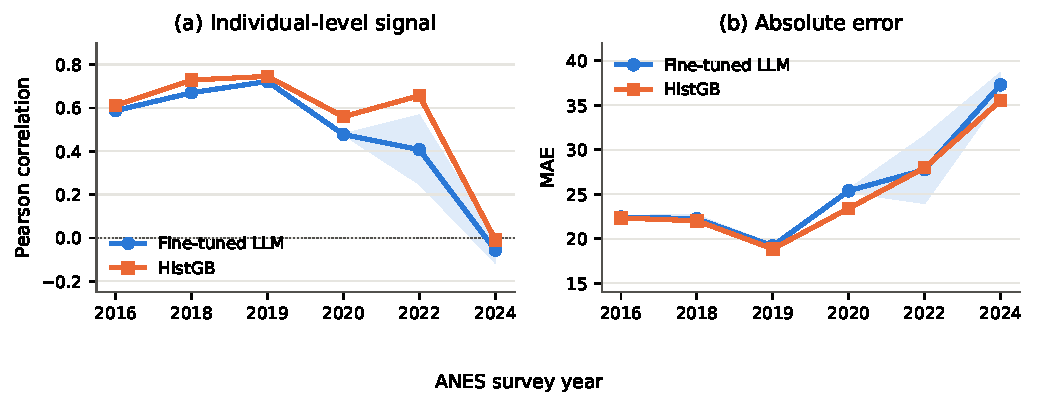
\includegraphics[width=\linewidth]{figures/fig2_temporal_decay.pdf}
\caption{Per-year correlation (a) and MAE (b) for the fine-tuned LLM and HistGB.
Shaded bands are standard deviations over three seeds.}
\label{fig:temporal}
\end{figure}

For the fine-tuned LLM, the correlation is 0.722 in 2019, 0.478 in 2020, 0.408 in
2022, and $-0.056$ in 2024; MAE rises from 19.20 to 25.39, 27.76, and 37.30.
HistGB decays later but collapses in the same way: 0.746, 0.560, 0.657, and
$-0.008$; MAE 18.85, 23.41, 27.98, and 35.52. The decay begins between 2019 and
2020, not at 2024. The LLM decays earlier than the tabular baseline: by 2022 its
correlation is 0.408 while HistGB is still at 0.657.

\section{The 2024 Collapse and a Failed Mitigation}

On the full 2024 test set the fine-tuned LLM reaches an MAE of 36.47 $\pm$ 0.75
but a correlation of $-0.029$ $\pm$ 0.021; HistGB reaches 35.06 and $-0.030$.
The predictions concentrate on the middle of the scale: 3,173 of 3,421 LLM
predictions are exactly 50, and every Biden row is predicted as 50 (standard
deviation 0.0), while Trump rows have a standard deviation of 17.4 and a
correlation of $-0.014$. The anchor readout does not rescue the signal: its
correlation is 0.003 with a prediction standard deviation of 2.1, so its low ECE
is an artefact of near-constant predictions. This is not LLM-specific: HistGB,
which has no language-model component, also loses the individual signal.

A natural mitigation is to add the most recent wave to training. The model is
fine-tuned on the union of the 2016--2020 pool and the 2022 validation rows
(9,017 rows) and evaluated on 2024. The result is unchanged: MAE 36.62,
correlation $-0.030$, choice 0.525. Adding 2022 does not restore the signal,
which points to a genuine distribution shift rather than a lack of recent data.

\section{Ablations}

Three design choices are isolated with matched runs. A1 replaces the nine-strategy
pool with a uniform random sample of the same size. A2 removes the interaction
block from the prompt. A3 additionally removes the candidate's party, position,
and age. All use seed 42 and the same in-distribution rows.

The full model reaches an MAE of 20.84 $\pm$ 0.24, a correlation of 0.679
$\pm$ 0.003, and a choice accuracy of 0.553 $\pm$ 0.011. A1 reaches 21.27, 0.658,
and 0.543; A2 reaches 21.13, 0.670, and 0.567; A3 reaches 21.45, 0.657, and
0.565. The direction is consistent but should be read as a small, descriptive
trend: removing the distribution-aware sampling or the candidate metadata worsens
MAE by roughly half a point and lowers correlation by about 0.02. Because each
ablation uses one seed, the thesis does not claim that each component is
individually necessary; the full table is in Appendix~\ref{app:results}.

The cross-pressure analysis gives a finer-grained view. The fine-tuned LLM is
substantially better than HistGB on CP3, the identity-versus-party conflict (MAE
15.51--17.80 versus 20.31), and comparable on CP1 (18.77--21.55 versus 21.55). It
is slightly worse on CP2 (23.21--24.13 versus 23.18) and on non-conflict rows
(20.45--21.09 versus 20.14). The cells are small, so the result is descriptive.

\chapter{Limitations and Conclusion}
\label{ch:conclusion}

\section{Limitations}

\textbf{Model and survey coverage.} All fine-tuning experiments use Qwen3-8B. A
second model family was not evaluated because the Llama-3.1-8B weights are gated
and the account used for this project was not authorized. The pipeline is
model-agnostic, but the empirical claims are conditional on Qwen3-8B. Both ANES
and GSS are from the United States; cross-national surveys, non-English
questionnaires, and non-political attitude domains are not tested.

\textbf{Group attitudes.} A nine-group voter--group corpus and two protocols were
constructed, but the group model was not evaluated. Group coverage is uneven
across waves (three groups in 2016, nine in 2020, two in 2022), and the 2020 block
lacks respondent identifiers. The claims are restricted to candidate-level PAS and
GSS FAS.

\textbf{Panel and choice metric.} ANES is a panel: there are no test-only
respondents in 2022/2024, and the T$\times$R cell is small (226 rows). No protocol
isolates a genuinely new respondent observed only in a future wave. Choice is
rating-induced: it is compared with the highest ground-truth thermometer score,
not with an observed vote.

\textbf{Ablations and FAS.} The ablations use one seed each; the effects are small
and the cross-pressure cells are small. FAS covers two three-attribute
configurations. EDC improves strongly; EHC improves less, and the joint symmetric
KL moves in the opposite direction for direct SFT. The temporal extrapolation is
validated only for 2024, and only one mitigation is tested.

\textbf{Ethics.} Synthetic respondents are not a substitute for real participants.
A model trained on historical data can reproduce and amplify the biases of that
data, and its outputs can be mistaken for evidence about a population. The
temporal results are a warning: a simulator that looks accurate in-distribution
can lose all individual signal four years later. Deployments should report the
training era, validation protocol, model family, and generated-sample coverage,
and synthetic results should be clearly labelled.

\section{Conclusion}

This thesis presented a data-centric pipeline for LLM survey simulation and
evaluated it at the individual, population, and temporal levels. The pipeline
reconstructs interaction-level ANES data, decouples candidate identity from
attributes, encodes partisan and ideological structure as explicit features,
samples the training pool to cover tails and conflict cases, and fine-tunes a
compact 8B model with LoRA. The same pipeline reconstructs a GSS joint
distribution and fine-tunes a model to generate a synthetic population.

The individual-level result is deliberately modest. On unseen respondents in the
same era, the fine-tuned model reaches an MAE of 20.84, a correlation of 0.679,
and a choice accuracy of 0.518 against chance 0.163. A gradient-boosted baseline
reaches 20.58, 0.714, and 0.534, and paired bootstrap shows no significant MAE or
choice difference. The value of the language model is not superior point
prediction; it is a unified interface that produces a rating distribution and
extends to population-level generation. The population-level result is stronger
for EDC: fine-tuning reduces marginal and joint JS divergence by 91\% and 86\%
(93\% and 82\% for the fully covered run).

The temporal result is the most important negative finding. Individual-level
correlation falls from 0.722 in 2019 to $-0.056$ in 2024, and the tabular baseline
collapses in the same way. Adding the most recent wave does not help. Structured
alignment is necessary but not sufficient for temporal generalization, and
temporal shift should be treated as a first-class evaluation axis. Future work
should replicate the pipeline on a second model family, extend it to
cross-national and group-attitude data, develop temporal adaptation methods, and
validate rating-induced choice against observed vote choice.


% ---------------------------------------------------------------------------
% Bibliography and appendices
% ---------------------------------------------------------------------------
\clearpage
\addcontentsline{toc}{chapter}{Bibliography}
\bibliographystyle{apalike}
\bibliography{references}

\appendix
\titleformat{\chapter}[display]
  {\normalfont\centering\bfseries\fontsize{14}{17}\selectfont}
  {APPENDIX \thechapter:}{0.5ex}{\fontsize{14}{17}\selectfont}
\chapter{Data Construction Details}
\label{app:data}

\section{Data Audit}

Table~\ref{tab:audit_full} reports the raw and cleaned row counts and the main
data defects. The trailing-period duplicates are normalized before deduplication;
the group-like targets are removed from the candidate table and kept in the group
corpus. The cleaned table retains the original row index so that every row can be
traced back to the raw ANES table.

\begin{table}[h]
\centering
\small
\begin{tabular}{lr}
\toprule
Item & Count \\
\midrule
Raw rows & 132,948 \\
Trailing-period duplicate rows & 8,165 \\
Group targets mixed into candidates & 23,060 \\
Missing or out-of-range scores & 3,588 \\
Duplicate rows removed after normalization & 8,141 \\
Clean rows & 98,159 \\
\bottomrule
\end{tabular}
\caption{Raw and cleaned row counts.}
\label{tab:audit_full}
\end{table}

\section{Splits}

\begin{table}[h]
\centering
\small
\begin{tabular}{llrr}
\toprule
Split & Years & Rows & Respondents \\
\midrule
\texttt{train\_t} & 2016--2020 & 6,516 & all \\
\texttt{val\_t} & 2022 & 2,501 & sampled \\
\texttt{test\_t} & 2024 & 3,421 & 1,712 \\
\texttt{train\_r} & 2016--2020 & 5,094 & 80\% \\
\texttt{test\_r} & 2016--2022 & 6,014 & 192 \\
\texttt{test\_tr} & 2024 & 226 & 113 \\
\bottomrule
\end{tabular}
\caption{Candidate splits. The two protocols are alternative designs and overlap
across each other; within each protocol the splits are disjoint.}
\label{tab:splits}
\end{table}

\section{Sampling Strategies}

The training pool is drawn with nine complementary strategies: balanced coverage
of the score range, hard cases near the middle of the scale, party-by-ideology
cells, similarity-stratified bins, cross-pressure cases, extreme scores,
incumbent effects, temporal coverage, and candidate-specific balance. The pool
contains 6,516 rows and is intentionally not a uniform sample; the test sets are
built from all cleaned rows in the target years so that evaluation is not shaped
by the same sampling design.

\section{Feature Definitions}

The core features are party match (+1 same party, $-1$ independent, 0 otherwise),
seven-point ideological distance, a composite demographic similarity index, and
three cross-pressure indicators: CP1 (same party, ideological distance $\ge3$),
CP2 (different party, distance $\le1$), and CP3 (similarity $\ge0.7$, different
party).

\chapter{Additional Results}
\label{app:results}

\section{Per-Year PAS Results}

\begin{table}[h]
\centering
\small
\caption{PAS by survey year on the held-out respondents. The 2022 and 2024 waves
have two candidates, so chance choice accuracy is 0.5.}
\label{tab:year_full}
\begin{tabular}{lccccccc}
\toprule
& & \multicolumn{3}{c}{Fine-tuned LLM} & \multicolumn{3}{c}{HistGB} \\
\cmidrule(lr){3-5}\cmidrule(lr){6-8}
Year & $n$ & MAE & corr & choice & MAE & corr & choice \\
\midrule
2016 & 697 & 22.45 & 0.588 & 0.329 & 22.32 & 0.611 & 0.256 \\
2018 & 727 & 22.25 & 0.670 & 0.530 & 22.02 & 0.729 & 0.544 \\
2019 & 1,302 & 19.20 & 0.722 & 0.663 & 18.85 & 0.746 & 0.639 \\
2020 & 2,868 & 25.39 & 0.478 & 0.326 & 23.41 & 0.560 & 0.278 \\
2022 & 194 & 27.76 & 0.408 & 0.674 & 27.98 & 0.657 & 0.804 \\
2024 & 226 & 37.30 & $-0.056$ & 0.448 & 35.52 & $-0.008$ & 0.460 \\
\bottomrule
\end{tabular}
\end{table}

\section{Ablations}

\begin{table}[h]
\centering
\small
\caption{Ablations on the 2016--2019 in-distribution rows.}
\label{tab:ablation_full}
\begin{tabular}{lccc}
\toprule
Configuration & MAE & Correlation & Choice \\
\midrule
Full (9-strategy) & 20.84 $\pm$ 0.24 & 0.679 $\pm$ 0.003 & 0.553 $\pm$ 0.011 \\
A1 random sampling & 21.27 & 0.658 & 0.543 \\
A2 minimal prompt & 21.13 & 0.670 & 0.567 \\
A3 name-only prompt & 21.45 & 0.657 & 0.565 \\
\bottomrule
\end{tabular}
\end{table}

\section{Cross-Pressure Subgroups}

\begin{table}[h]
\centering
\small
\caption{Cross-pressure subgroups on the 2016--2019 rows.}
\label{tab:cp_full}
\begin{tabular}{lccc}
\toprule
Subgroup & LLM MAE (3 seeds) & HistGB MAE & $n$ \\
\midrule
CP1 party vs.\ ideology & 18.77--21.55 & 21.55 & 154 \\
CP2 ideology vs.\ party & 23.21--24.13 & 23.18 & 318 \\
CP3 identity vs.\ party & 15.51--17.80 & 20.31 & 164 \\
No conflict & 20.45--21.09 & 20.14 & 2,090 \\
\bottomrule
\end{tabular}
\end{table}

\chapter{FAS Details}
\label{app:fas}

\section{Full FAS Table}

\begin{table}[h]
\centering
\small
\caption{FAS distributional alignment on GSS (JS divergence, lower is better).
Coverage is the fraction of the 400 requested rows returned.}
\label{tab:fas_full}
\begin{tabular}{llcccc}
\toprule
Config & Run & $n$ & Coverage & Marginal JS & Joint JS \\
\midrule
\multirow{6}{*}{EDC} & Base & 400 & 1.000 & 0.0552 & 0.1181 \\
 & SFT & 381 & 0.953 & 0.0048 & 0.0160 \\
 & SFT (v3) & 400 & 1.000 & \textbf{0.0040} & 0.0215 \\
 & RAG & 376 & 0.940 & 0.0473 & 0.1096 \\
 & RAG + SFT & 381 & 0.953 & 0.0054 & 0.0176 \\
 & Quota & 395 & 0.988 & 0.0091 & 0.0216 \\
\midrule
\multirow{6}{*}{EHC} & Base & 351 & 0.877 & 0.0319 & 0.1001 \\
 & SFT & 400 & 1.000 & 0.0167 & 0.0470 \\
 & SFT (v3) & 400 & 1.000 & \textbf{0.0077} & \textbf{0.0363} \\
 & RAG & 379 & 0.948 & 0.0404 & 0.1095 \\
 & RAG + SFT & 380 & 0.950 & 0.0152 & 0.0427 \\
 & Quota & 400 & 1.000 & 0.0175 & 0.0522 \\
\bottomrule
\end{tabular}
\end{table}

\section{Bootstrap Confidence Intervals}

\begin{table}[h]
\centering
\small
\resizebox{\linewidth}{!}{%
\begin{tabular}{llcccc}
\toprule
Config & Run & Marginal JS [95\% CI] & Joint JS [95\% CI] \\
\midrule
EDC & Base & 0.0552 [0.0476, 0.0644] & 0.1181 [0.1035, 0.1371] \\
 & SFT & 0.0048 [0.0029, 0.0089] & 0.0160 [0.0139, 0.0247] \\
 & SFT-v3 & 0.0040 [0.0022, 0.0077] & 0.0215 [0.0181, 0.0305] \\
EHC & Base & 0.0319 [0.0260, 0.0400] & 0.1001 [0.0874, 0.1188] \\
 & SFT & 0.0167 [0.0130, 0.0229] & 0.0470 [0.0413, 0.0587] \\
 & SFT-v3 & 0.0077 [0.0052, 0.0123] & 0.0363 [0.0332, 0.0458] \\
\bottomrule
\end{tabular}}
\caption{Bootstrap 95\% CIs from 1,000 resamples of the generated rows.}
\label{tab:fas_ci}
\end{table}

\section{Prompt Templates}

For PAS, the system message defines the task and fixes the output format; the
user message contains the voter profile, the candidate block, and the interaction
block. A representative user message is:

\begin{quote}\small
Predict the support score (0--100) for this voter--candidate pair.

Voter Profile: 45-year-old Female White; Bachelor's degree; Strong Democrat,
Liberal.

Candidate: Biden; Democrat; President; Age 78.

Key Interactions: Same party; Ideology distance 0.5; Age difference 33 years;
Year 2020.

Support score (0--100):
\end{quote}

For FAS, the model is given the target year, the three attributes and their
levels, and the task type (batch generation, prior sampling, scenario variation,
subgroup analysis, or iterative correction). The expected output is a list of
rows, one per synthetic respondent.

\section{Hyperparameters}

\begin{table}[h]
\centering
\small
\caption{Training and generation hyperparameters.}
\label{tab:hyper}
\begin{tabular}{ll}
\toprule
Parameter & Value \\
\midrule
Base model & Qwen3-8B \\
LoRA rank / alpha / dropout & 8 / 32 / 0.1 \\
Epochs & 3 \\
Learning rate & $10^{-4}$ \\
Effective batch size & 16 \\
Maximum sequence length & 512 \\
Seeds & 42, 43, 44 \\
IPF iterations & 800 \\
FAS target samples & 400 \\
\bottomrule
\end{tabular}
\end{table}


\chapter*{Vita}
\addcontentsline{toc}{chapter}{Vita}
CHENYU YUAN received the degree of Master of Computer Science from the
University of Macau in April 2027. Her research interests include large language
models, computational social science, and survey simulation.

\end{document}
